\documentclass[]{article}
\usepackage{lmodern}
\usepackage{amssymb,amsmath}
\usepackage{ifxetex,ifluatex}
\usepackage{fixltx2e} % provides \textsubscript
\ifnum 0\ifxetex 1\fi\ifluatex 1\fi=0 % if pdftex
  \usepackage[T1]{fontenc}
  \usepackage[utf8]{inputenc}
\else % if luatex or xelatex
  \ifxetex
    \usepackage{mathspec}
  \else
    \usepackage{fontspec}
  \fi
  \defaultfontfeatures{Ligatures=TeX,Scale=MatchLowercase}
\fi
% use upquote if available, for straight quotes in verbatim environments
\IfFileExists{upquote.sty}{\usepackage{upquote}}{}
% use microtype if available
\IfFileExists{microtype.sty}{%
\usepackage{microtype}
\UseMicrotypeSet[protrusion]{basicmath} % disable protrusion for tt fonts
}{}
\usepackage[margin=1in]{geometry}
\usepackage{hyperref}
\hypersetup{unicode=true,
            pdftitle={The OmicsPLS R Package},
            pdfauthor={Said el Bouhaddani},
            pdfborder={0 0 0},
            breaklinks=true}
\urlstyle{same}  % don't use monospace font for urls
\usepackage{color}
\usepackage{fancyvrb}
\newcommand{\VerbBar}{|}
\newcommand{\VERB}{\Verb[commandchars=\\\{\}]}
\DefineVerbatimEnvironment{Highlighting}{Verbatim}{commandchars=\\\{\}}
% Add ',fontsize=\small' for more characters per line
\usepackage{framed}
\definecolor{shadecolor}{RGB}{248,248,248}
\newenvironment{Shaded}{\begin{snugshade}}{\end{snugshade}}
\newcommand{\KeywordTok}[1]{\textcolor[rgb]{0.13,0.29,0.53}{\textbf{{#1}}}}
\newcommand{\DataTypeTok}[1]{\textcolor[rgb]{0.13,0.29,0.53}{{#1}}}
\newcommand{\DecValTok}[1]{\textcolor[rgb]{0.00,0.00,0.81}{{#1}}}
\newcommand{\BaseNTok}[1]{\textcolor[rgb]{0.00,0.00,0.81}{{#1}}}
\newcommand{\FloatTok}[1]{\textcolor[rgb]{0.00,0.00,0.81}{{#1}}}
\newcommand{\ConstantTok}[1]{\textcolor[rgb]{0.00,0.00,0.00}{{#1}}}
\newcommand{\CharTok}[1]{\textcolor[rgb]{0.31,0.60,0.02}{{#1}}}
\newcommand{\SpecialCharTok}[1]{\textcolor[rgb]{0.00,0.00,0.00}{{#1}}}
\newcommand{\StringTok}[1]{\textcolor[rgb]{0.31,0.60,0.02}{{#1}}}
\newcommand{\VerbatimStringTok}[1]{\textcolor[rgb]{0.31,0.60,0.02}{{#1}}}
\newcommand{\SpecialStringTok}[1]{\textcolor[rgb]{0.31,0.60,0.02}{{#1}}}
\newcommand{\ImportTok}[1]{{#1}}
\newcommand{\CommentTok}[1]{\textcolor[rgb]{0.56,0.35,0.01}{\textit{{#1}}}}
\newcommand{\DocumentationTok}[1]{\textcolor[rgb]{0.56,0.35,0.01}{\textbf{\textit{{#1}}}}}
\newcommand{\AnnotationTok}[1]{\textcolor[rgb]{0.56,0.35,0.01}{\textbf{\textit{{#1}}}}}
\newcommand{\CommentVarTok}[1]{\textcolor[rgb]{0.56,0.35,0.01}{\textbf{\textit{{#1}}}}}
\newcommand{\OtherTok}[1]{\textcolor[rgb]{0.56,0.35,0.01}{{#1}}}
\newcommand{\FunctionTok}[1]{\textcolor[rgb]{0.00,0.00,0.00}{{#1}}}
\newcommand{\VariableTok}[1]{\textcolor[rgb]{0.00,0.00,0.00}{{#1}}}
\newcommand{\ControlFlowTok}[1]{\textcolor[rgb]{0.13,0.29,0.53}{\textbf{{#1}}}}
\newcommand{\OperatorTok}[1]{\textcolor[rgb]{0.81,0.36,0.00}{\textbf{{#1}}}}
\newcommand{\BuiltInTok}[1]{{#1}}
\newcommand{\ExtensionTok}[1]{{#1}}
\newcommand{\PreprocessorTok}[1]{\textcolor[rgb]{0.56,0.35,0.01}{\textit{{#1}}}}
\newcommand{\AttributeTok}[1]{\textcolor[rgb]{0.77,0.63,0.00}{{#1}}}
\newcommand{\RegionMarkerTok}[1]{{#1}}
\newcommand{\InformationTok}[1]{\textcolor[rgb]{0.56,0.35,0.01}{\textbf{\textit{{#1}}}}}
\newcommand{\WarningTok}[1]{\textcolor[rgb]{0.56,0.35,0.01}{\textbf{\textit{{#1}}}}}
\newcommand{\AlertTok}[1]{\textcolor[rgb]{0.94,0.16,0.16}{{#1}}}
\newcommand{\ErrorTok}[1]{\textcolor[rgb]{0.64,0.00,0.00}{\textbf{{#1}}}}
\newcommand{\NormalTok}[1]{{#1}}
\usepackage{graphicx,grffile}
\makeatletter
\def\maxwidth{\ifdim\Gin@nat@width>\linewidth\linewidth\else\Gin@nat@width\fi}
\def\maxheight{\ifdim\Gin@nat@height>\textheight\textheight\else\Gin@nat@height\fi}
\makeatother
% Scale images if necessary, so that they will not overflow the page
% margins by default, and it is still possible to overwrite the defaults
% using explicit options in \includegraphics[width, height, ...]{}
\setkeys{Gin}{width=\maxwidth,height=\maxheight,keepaspectratio}
\IfFileExists{parskip.sty}{%
\usepackage{parskip}
}{% else
\setlength{\parindent}{0pt}
\setlength{\parskip}{6pt plus 2pt minus 1pt}
}
\setlength{\emergencystretch}{3em}  % prevent overfull lines
\providecommand{\tightlist}{%
  \setlength{\itemsep}{0pt}\setlength{\parskip}{0pt}}
\setcounter{secnumdepth}{0}
% Redefines (sub)paragraphs to behave more like sections
\ifx\paragraph\undefined\else
\let\oldparagraph\paragraph
\renewcommand{\paragraph}[1]{\oldparagraph{#1}\mbox{}}
\fi
\ifx\subparagraph\undefined\else
\let\oldsubparagraph\subparagraph
\renewcommand{\subparagraph}[1]{\oldsubparagraph{#1}\mbox{}}
\fi

%%% Use protect on footnotes to avoid problems with footnotes in titles
\let\rmarkdownfootnote\footnote%
\def\footnote{\protect\rmarkdownfootnote}

%%% Change title format to be more compact
\usepackage{titling}

% Create subtitle command for use in maketitle
\newcommand{\subtitle}[1]{
  \posttitle{
    \begin{center}\large#1\end{center}
    }
}

\setlength{\droptitle}{-2em}
  \title{The OmicsPLS R Package}
  \pretitle{\vspace{\droptitle}\centering\huge}
  \posttitle{\par}
  \author{Said el Bouhaddani}
  \preauthor{\centering\large\emph}
  \postauthor{\par}
  \predate{\centering\large\emph}
  \postdate{\par}
  \date{2017-04-24}


\begin{document}
\maketitle

\section{The OmicsPLS R package}\label{the-omicspls-r-package}

Welcome to the vignette of the O2PLS package for analyzing two Omics
datasets!

Here you can find examples and explanation of the input options and
output objects. As always: help is always found by using the \texttt{?}
operator. Try to type \texttt{?OmicsPLS} for an overview of the package
and \texttt{?o2m} for description of the main fitting function.

\subsection{Background}\label{background}

\subsubsection{The O2PLS method}\label{the-o2pls-method}

The O2PLS method is proposed in (Trygg \& Wold, 2003). It decomposes the
variation of two datasets in three parts:

\begin{itemize}
\tightlist
\item
  A Joint part for \(X\) and \(Y\): \(TW^\top\) and \(UC^\top\),
\item
  A Systematic/Specific/Orthogonal part for \(X\) and \(Y\):
  \(T_\perp W_\perp^\top\) and \(U_\perp C_\perp^\top\),
\item
  A noise part for \(X\) and \(Y\): \(E\) and \(F\).
\end{itemize}

The number of columns in \(T\), \(U\), \(W\) and \(C\) are denoted by as
\(n\) and are referred to as the number of joint components. The number
of columns in \(T_\perp\) and \(W_\perp\) are denoted by as \(n_X\) and
are referred to as the number of \(X\)-specific components. Analoguous
for \(Y\), where we use \(n_Y\) to denote the number of \(Y\)-specific
components. The relation between \(T\) and \(U\) makes the joint part
the joint part: \(U = TB + H\) or \(U = TB'+ H'\). The number of
components \((n, n_X, n_Y)\) are chosen beforehand (e.g.~with
Cross-Validation).

\subsubsection{Cross-Validation}\label{cross-validation}

In cross-validation (CV) one minimizes a certain measure of error over
some parameters that should be determined a priori. In our case we have
three parameters: \((n, n_X, n_Y)\). A popular measure is the prediction
error \(||\hat{Y} - Y||\), where \(\hat{Y}\) is a prediction of \(Y\).
In our case the O2PLS method is symmetric in \(X\) and \(Y\), so we
minimize the sum of the prediction errors:
\(||\hat{X} - X||+||\hat{Y} - Y||\). The idea is to fit O2PLS to our
data \(X\) and \(Y\) and compute the prediction errors for a grid of
values for \(n\), \(n_X\) and \(n_Y\). Here \(n\) should be a positive
integer, and \(n_X\) and \(n_Y\) should be non-negative. The `best'
integers are then the minimizers of the prediction error.

\subsubsection{Proposed cross-validation
approach}\label{proposed-cross-validation-approach}

We proposed an alternative way for choosing the number of components (el
Bouhaddani, 2016). Here we construct a grid of values for \(n\). For
each \(n\) we consider then the \(R^2\) between \(T\) and \(U\) for
different \(n_X\) and \(n_Y\). If \(T\) and \(U\) are contaminated with
data-specific variation the \(R^2\) will be lower. If too many specific
components are removed the \(R^2\) will again be lower. Somewhere in
between is the maximum, with its maximizers \(n_X\) and \(n_Y\). With
these two integers we now compute the prediction error for our \(n\)
that we have kept fixed. This process we repeat for each \(n\) on the
one-dimensional grid and get our maximizers. This can provide a (big)
speed-up and often yields similar values for \((n, n_X, n_Y)\).

\subsection{Installing and loading}\label{installing-and-loading}

The easiest way is to run
\texttt{devtools::install\_github("selbouhaddani/OmicsPLS")}. If this
doesn't work, check if there is a package missing. It imports the
\textbf{ggplot2} and \textbf{parallel} package, so these should be
installed first. If there still is an error, try to download the .tar or
.zip (for Windows) and install offline. These two files can be found
also in the \emph{selbouhaddani/ZippedPackage} repository. Also feel
free to send an email with the error message you are receiving.

The OmicsPLS package is loaded by running \texttt{library(OmicsPLS)}.
Maybe you get a message saying that the \texttt{loadings} object is
masked from \texttt{package::stats}. This basically means that whenever
you type \texttt{loadings} (which is generic), you'll get the
\texttt{loadings.o2m} variant.

\subsection{A first test case}\label{a-first-test-case}

First we generate some data

\begin{Shaded}
\begin{Highlighting}[]
\KeywordTok{set.seed}\NormalTok{(564785412L)}
\NormalTok{X =}\StringTok{ }\KeywordTok{rnorm}\NormalTok{(}\DecValTok{100}\NormalTok{) %*%}\StringTok{ }\KeywordTok{t}\NormalTok{(}\KeywordTok{c}\NormalTok{(}\KeywordTok{rep}\NormalTok{(}\DecValTok{1}\NormalTok{,}\DecValTok{5}\NormalTok{), }\KeywordTok{rep}\NormalTok{(}\DecValTok{0}\NormalTok{,}\DecValTok{45}\NormalTok{))/}\KeywordTok{sqrt}\NormalTok{(}\DecValTok{5}\NormalTok{)) +}\StringTok{ }\CommentTok{# Component 1 = joint}
\StringTok{  }\KeywordTok{rnorm}\NormalTok{(}\DecValTok{100}\NormalTok{) %*%}\StringTok{ }\KeywordTok{t}\NormalTok{(}\KeywordTok{c}\NormalTok{(}\KeywordTok{rep}\NormalTok{(}\DecValTok{0}\NormalTok{,}\DecValTok{45}\NormalTok{), }\KeywordTok{rep}\NormalTok{(}\DecValTok{1}\NormalTok{,}\DecValTok{5}\NormalTok{))/}\KeywordTok{sqrt}\NormalTok{(}\DecValTok{5}\NormalTok{)) }\CommentTok{# Component 2 = specific}
\NormalTok{Y =}\StringTok{ }\NormalTok{X[,}\KeywordTok{c}\NormalTok{(}\DecValTok{6}\NormalTok{:}\DecValTok{25}\NormalTok{, }\DecValTok{1}\NormalTok{:}\DecValTok{5}\NormalTok{, }\DecValTok{26}\NormalTok{:}\DecValTok{45}\NormalTok{)] }\CommentTok{# Reorder columns of X and leave out last 5}
\NormalTok{X =}\StringTok{ }\NormalTok{X +}\StringTok{ }\KeywordTok{matrix}\NormalTok{(}\KeywordTok{rnorm}\NormalTok{(}\DecValTok{100}\NormalTok{*}\DecValTok{50}\NormalTok{), }\DataTypeTok{nrow=}\DecValTok{100}\NormalTok{) }\CommentTok{# add noise}
\NormalTok{Y =}\StringTok{ }\NormalTok{Y +}\StringTok{ }\KeywordTok{matrix}\NormalTok{(}\KeywordTok{rnorm}\NormalTok{(}\DecValTok{100}\NormalTok{*}\DecValTok{45}\NormalTok{), }\DataTypeTok{nrow=}\DecValTok{100}\NormalTok{) }\CommentTok{# add noise}

\NormalTok{X =}\StringTok{ }\KeywordTok{scale}\NormalTok{(X, }\DataTypeTok{scale=}\NormalTok{F)}
\NormalTok{Y =}\StringTok{ }\KeywordTok{scale}\NormalTok{(Y, }\DataTypeTok{scale=}\NormalTok{F)}
\end{Highlighting}
\end{Shaded}

Now \texttt{X} has 100 rows and 50 columns while \texttt{Y} has 100 rows
and 45 columns. We used two latent components in \(X\), which are hidden
in the first five and last five variables. The first five variables are
also present in \(Y_{20}\) to \(Y_{25}\). We add noise so we do not
exactly observe the latent structures.

We will use the \texttt{gplots} package to create heatmaps of
correlations.

\begin{Shaded}
\begin{Highlighting}[]
\KeywordTok{try}\NormalTok{(}
  \NormalTok{gplots::}\KeywordTok{heatmap.2}\NormalTok{(}\KeywordTok{cor}\NormalTok{(X,Y), }\DataTypeTok{Rowv=}\NormalTok{F,}\DataTypeTok{Colv=}\NormalTok{F, }\DataTypeTok{col=}\NormalTok{gplots::}\KeywordTok{bluered}\NormalTok{(}\DecValTok{100}\NormalTok{)),}
  \DataTypeTok{silent =} \OtherTok{TRUE}\NormalTok{)}
\end{Highlighting}
\end{Shaded}

\begin{verbatim}
## Warning in gplots::heatmap.2(cor(X, Y), Rowv = F, Colv = F, col =
## gplots::bluered(100)): Discrepancy: Rowv is FALSE, while dendrogram is
## `both'. Omitting row dendogram.
\end{verbatim}

\begin{verbatim}
## Warning in gplots::heatmap.2(cor(X, Y), Rowv = F, Colv = F, col =
## gplots::bluered(100)): Discrepancy: Colv is FALSE, while dendrogram is
## `column'. Omitting column dendogram.
\end{verbatim}

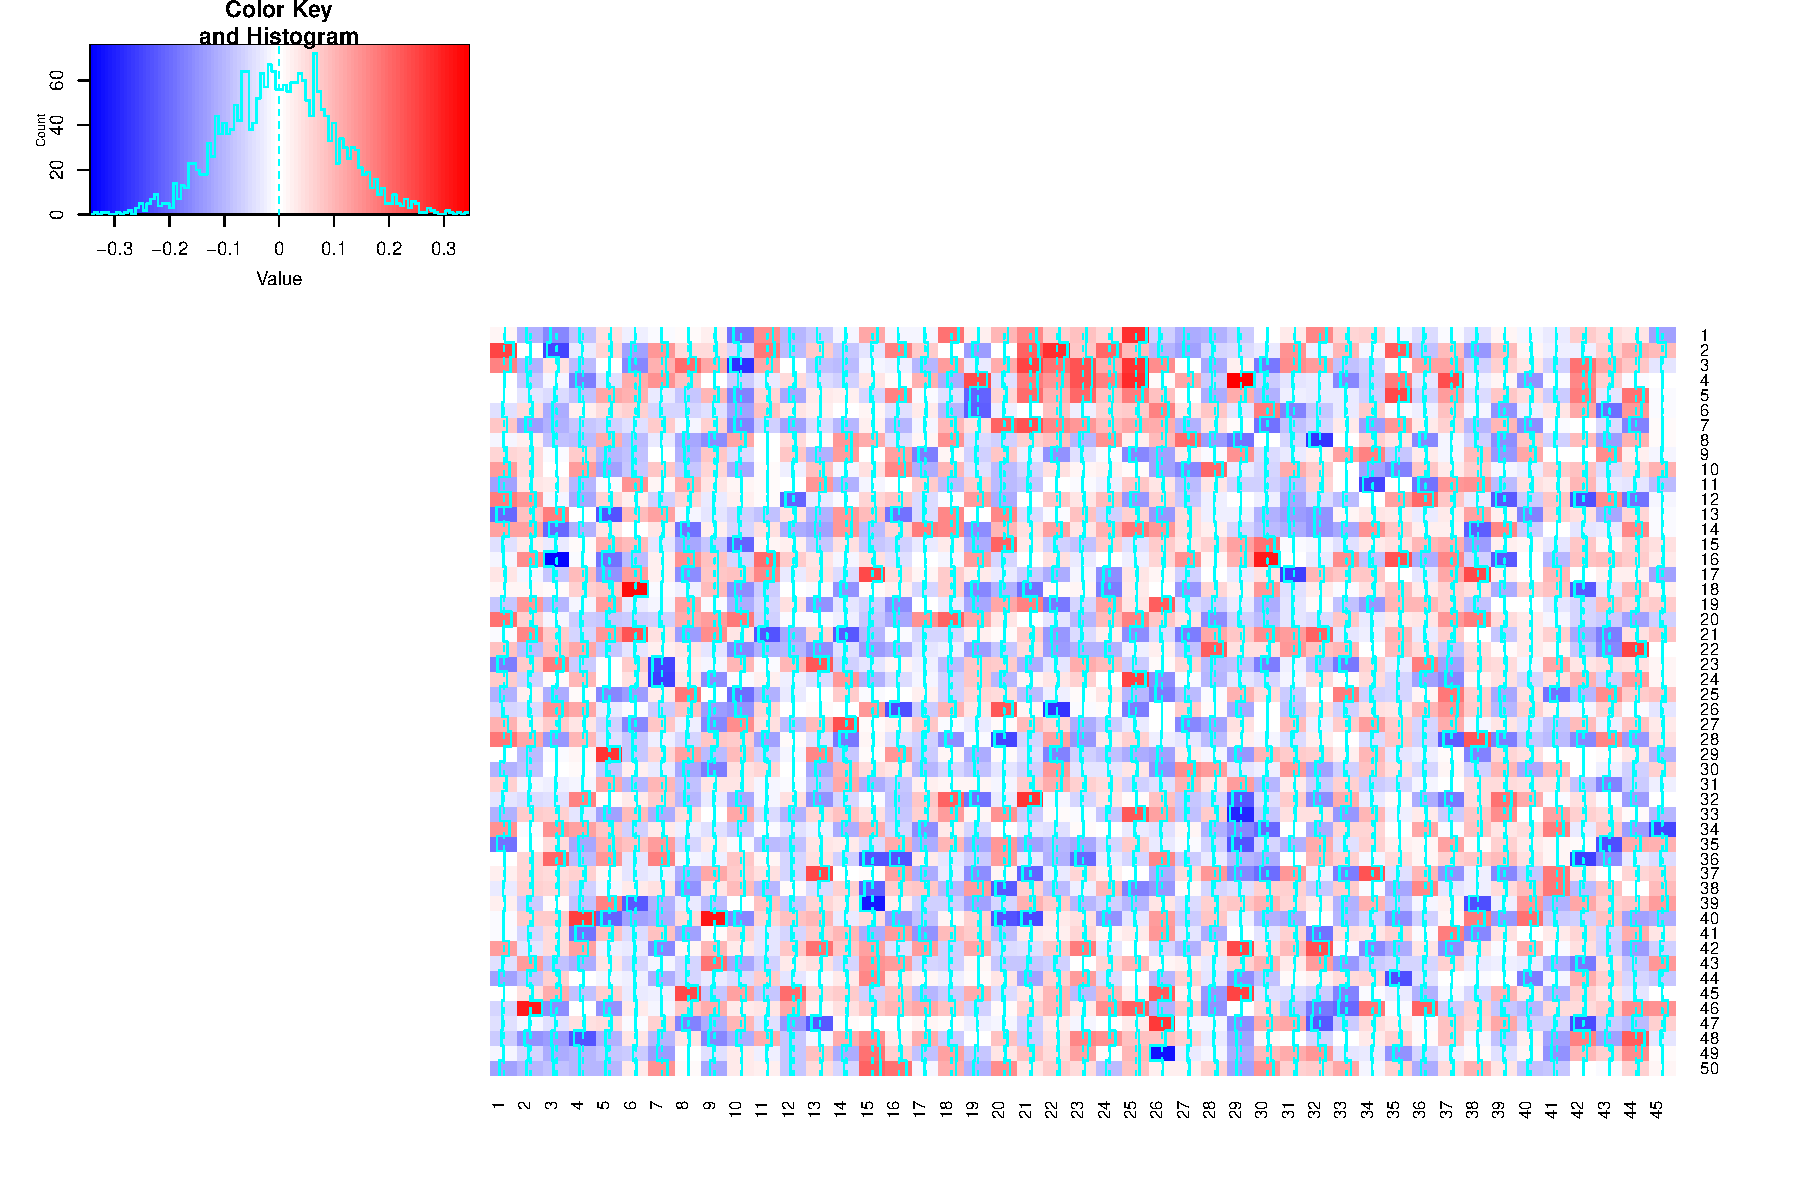
\includegraphics{Figs/unnamed-chunk-2-1.pdf} It is difficult to see
where the correlated part lies. We will try to find out with O2PLS.
First we need to determine the number of components.

\begin{Shaded}
\begin{Highlighting}[]
\KeywordTok{library}\NormalTok{(OmicsPLS)}
\KeywordTok{set.seed}\NormalTok{(1221L)}
\KeywordTok{crossval_o2m_adjR2}\NormalTok{(X, Y, }\DecValTok{1}\NormalTok{:}\DecValTok{3}\NormalTok{, }\DecValTok{0}\NormalTok{:}\DecValTok{3}\NormalTok{, }\DecValTok{0}\NormalTok{:}\DecValTok{3}\NormalTok{, }\DataTypeTok{nr_folds =} \DecValTok{2}\NormalTok{)}
\end{Highlighting}
\end{Shaded}

\begin{verbatim}
## minimum is at n = 1
\end{verbatim}

\begin{verbatim}
## Elapsed time: 0.36 sec
\end{verbatim}

\begin{verbatim}
##        MSE n nx ny
## 1 2.030027 1  1  1
## 2 2.053605 2  3  3
## 3 2.083403 3  3  3
\end{verbatim}

\begin{Shaded}
\begin{Highlighting}[]
\KeywordTok{crossval_o2m}\NormalTok{(X, Y, }\DecValTok{1}\NormalTok{:}\DecValTok{3}\NormalTok{, }\DecValTok{0}\NormalTok{:}\DecValTok{3}\NormalTok{, }\DecValTok{0}\NormalTok{:}\DecValTok{3}\NormalTok{, }\DataTypeTok{nr_folds =} \DecValTok{10}\NormalTok{)}
\end{Highlighting}
\end{Shaded}

\begin{verbatim}
## *******************
## Elapsed time: 2.55 sec
## *******
## Minimal 10-CV error is at ax=0 ay=1 a=1 
## *******
## Minimum is 2.022266 
## *******************
\end{verbatim}

The alternative cross-validation suggests one component in all parts.
The full cross-validation suggests one joint and one \(X\)-specific
component. Although the full CV got it right, the alternative yielded
similar answers in much less CPU time. This is partly because we use
more folds, but decreasing the number of folds to two yielded unreliable
results for the full CV.

We now fit the O2PLS model.

\begin{Shaded}
\begin{Highlighting}[]
\NormalTok{fit0 =}\StringTok{ }\KeywordTok{o2m}\NormalTok{(X, Y, }\DecValTok{1}\NormalTok{, }\DecValTok{1}\NormalTok{, }\DecValTok{0}\NormalTok{)}
\NormalTok{fit0}
\end{Highlighting}
\end{Shaded}

\begin{verbatim}
## O2PLS fit 
## with 1 joint components  
## and  1 orthogonal components in X 
## and  0 orthogonal components in Y 
## Elapsed time: 0 sec
\end{verbatim}

\begin{Shaded}
\begin{Highlighting}[]
\KeywordTok{summary}\NormalTok{(fit0)}
\end{Highlighting}
\end{Shaded}

\begin{verbatim}
## 
## *** Summary of the O2PLS fit *** 
## 
## -  Call: o2m(X = X, Y = Y, n = 1, nx = 1, ny = 0) 
## 
## -  Modeled variation
## -- Total variation:
## in X: 5100.552 
## in Y: 4576.141 
## 
## -- Joint, Orthogonal and Noise as proportions:
## 
##            data X data Y
## Joint       0.040  0.054
## Orthogonal  0.042  0.000
## Noise       0.918  0.946
## 
## -- Predictable variation in Y-joint part by X-joint part:
## Variation in Yhat relative to U: 0.693 
## -- Predictable variation in X-joint part by Y-joint part:
## Variation in Xhat relative to T: 0.693 
## 
## -- Variances per component:
## 
##          Comp 1
## X joint 206.273
## Y joint 247.776
## 
##         Comp 1
## X Orth 212.371
## 
## 
## -  Coefficient in 'U = T B_T + H_U' model:
## -- Diagonal elements of B_T =
##  0.912
\end{verbatim}

We can see that there is a lot of noise (92\% and 95\%), and only about
5\% joint variation. However relative to this variation, 69\% is
predictable. To see which variables induce the joint variation, we plot
the joint loadings of \(X\) and \(Y\).

\begin{Shaded}
\begin{Highlighting}[]
\KeywordTok{plot}\NormalTok{(fit0)}
\end{Highlighting}
\end{Shaded}

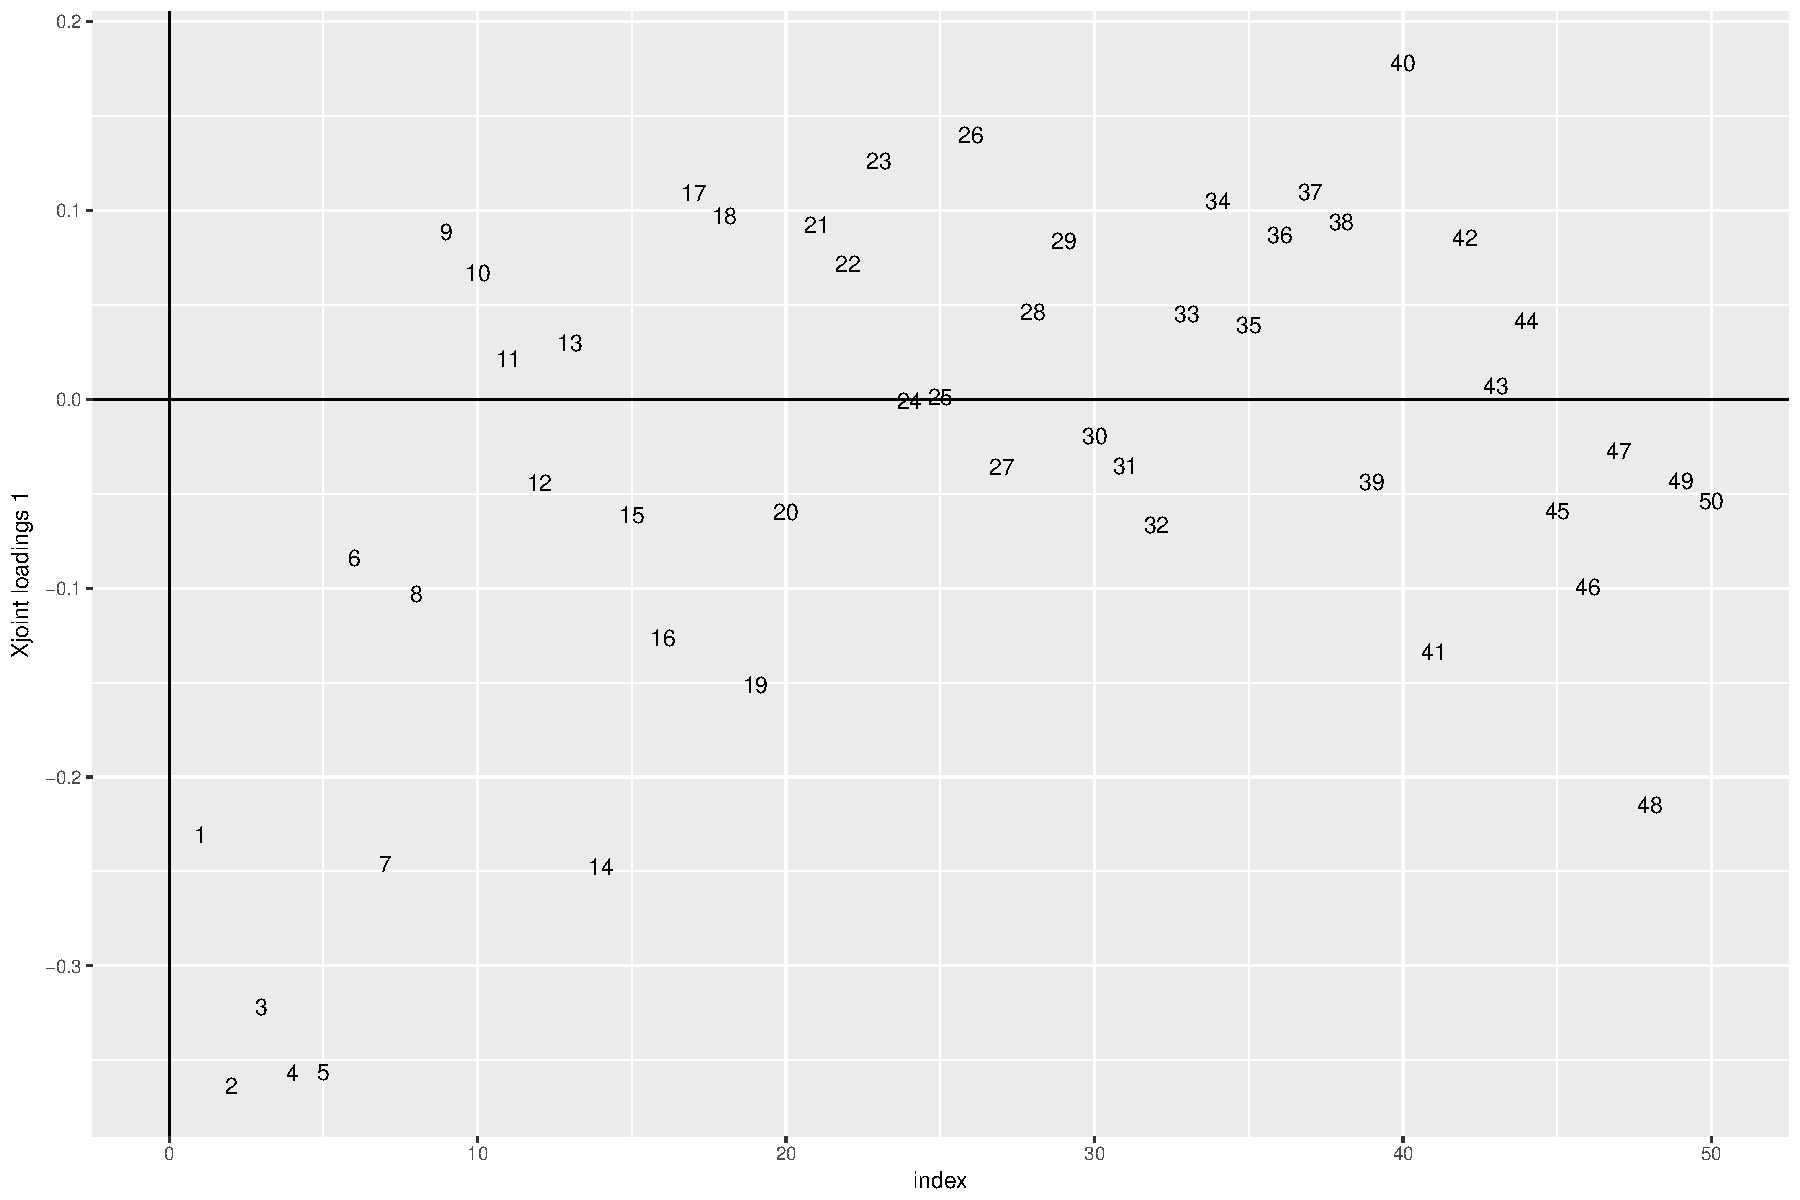
\includegraphics{Figs/unnamed-chunk-5-1.pdf}

\begin{Shaded}
\begin{Highlighting}[]
\KeywordTok{plot}\NormalTok{(fit0, }\StringTok{"Yj"}\NormalTok{)}
\end{Highlighting}
\end{Shaded}

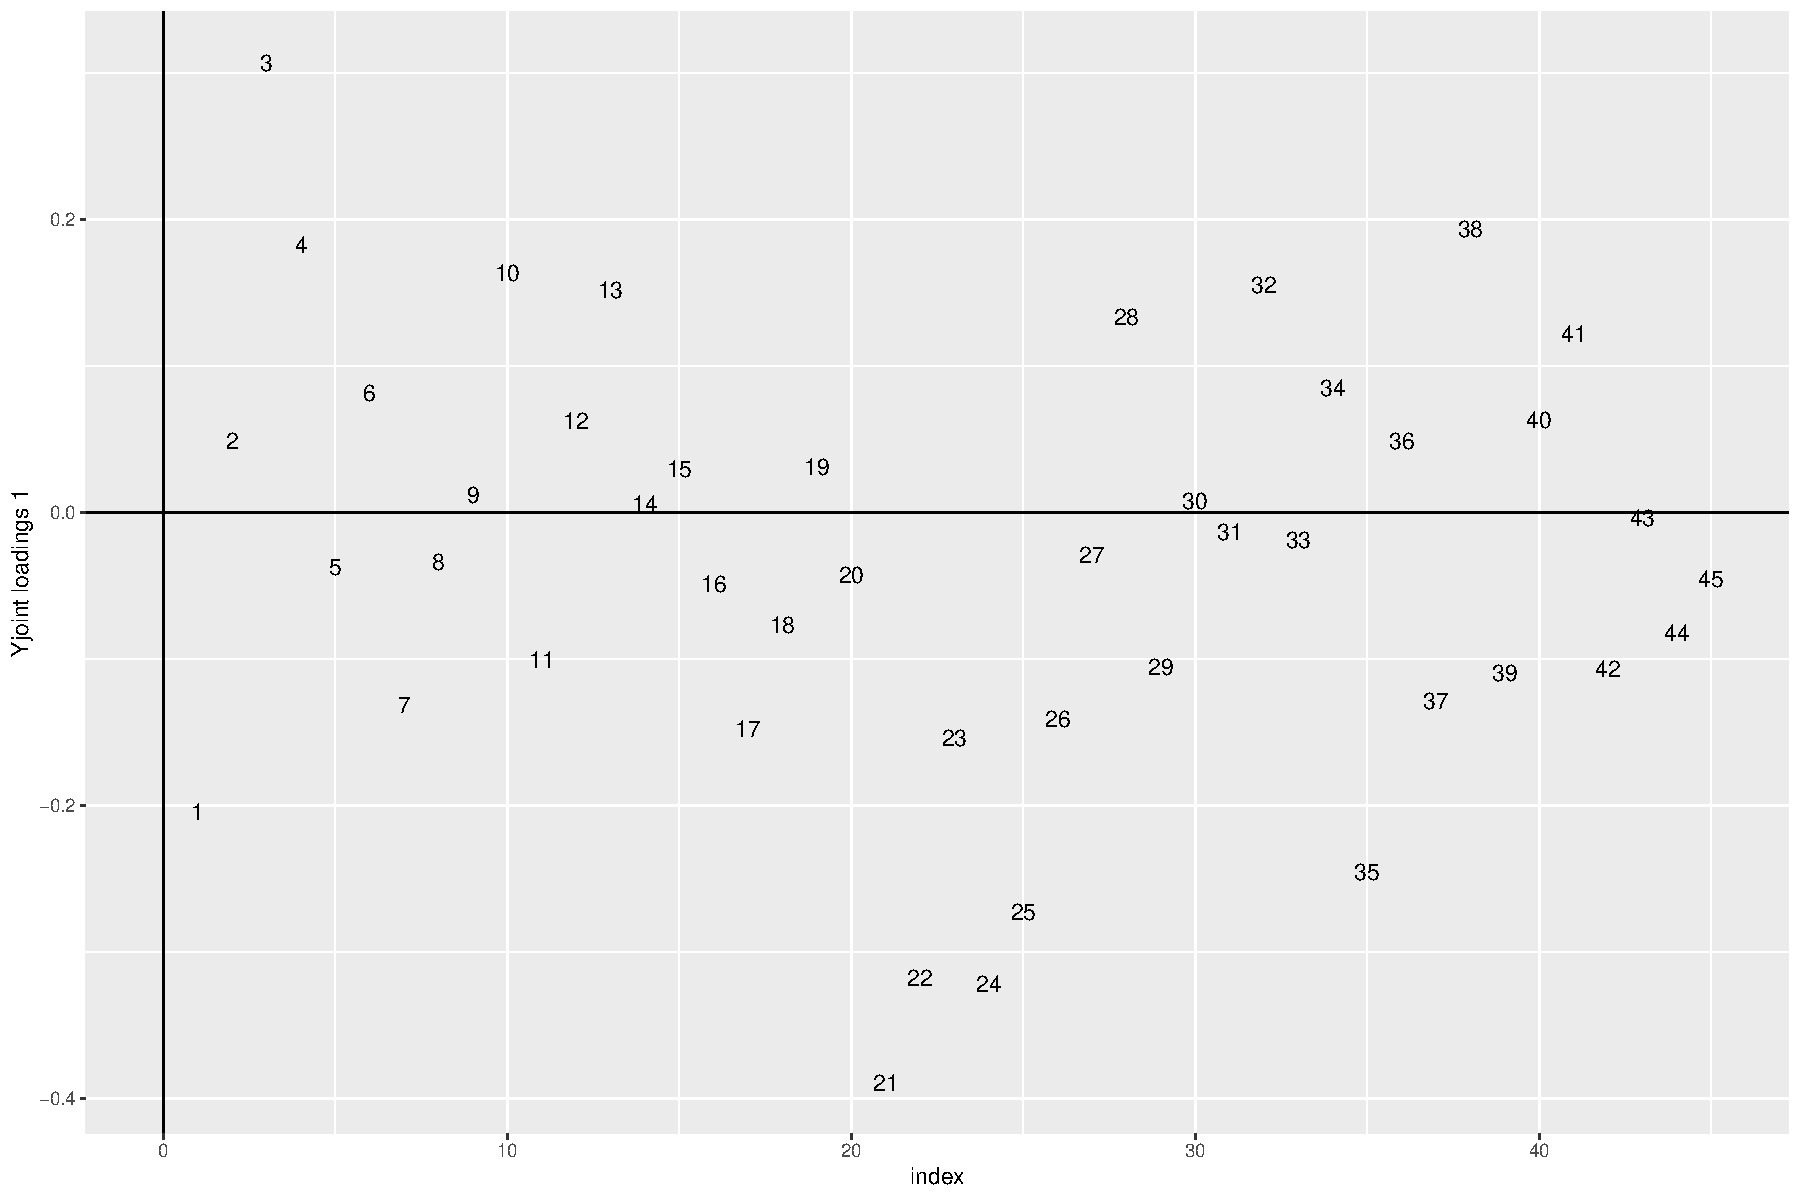
\includegraphics{Figs/unnamed-chunk-5-2.pdf} We see that more or less
the first five \(X\) variables and columns 21 to 25 of \(Y\) have high
absolute loading values.

The \(X\)-specific loadings are not recovered unfortunately, probably
due to the high noise level.

\begin{Shaded}
\begin{Highlighting}[]
\KeywordTok{plot}\NormalTok{(fit0, }\StringTok{"Xo"}\NormalTok{)}
\end{Highlighting}
\end{Shaded}

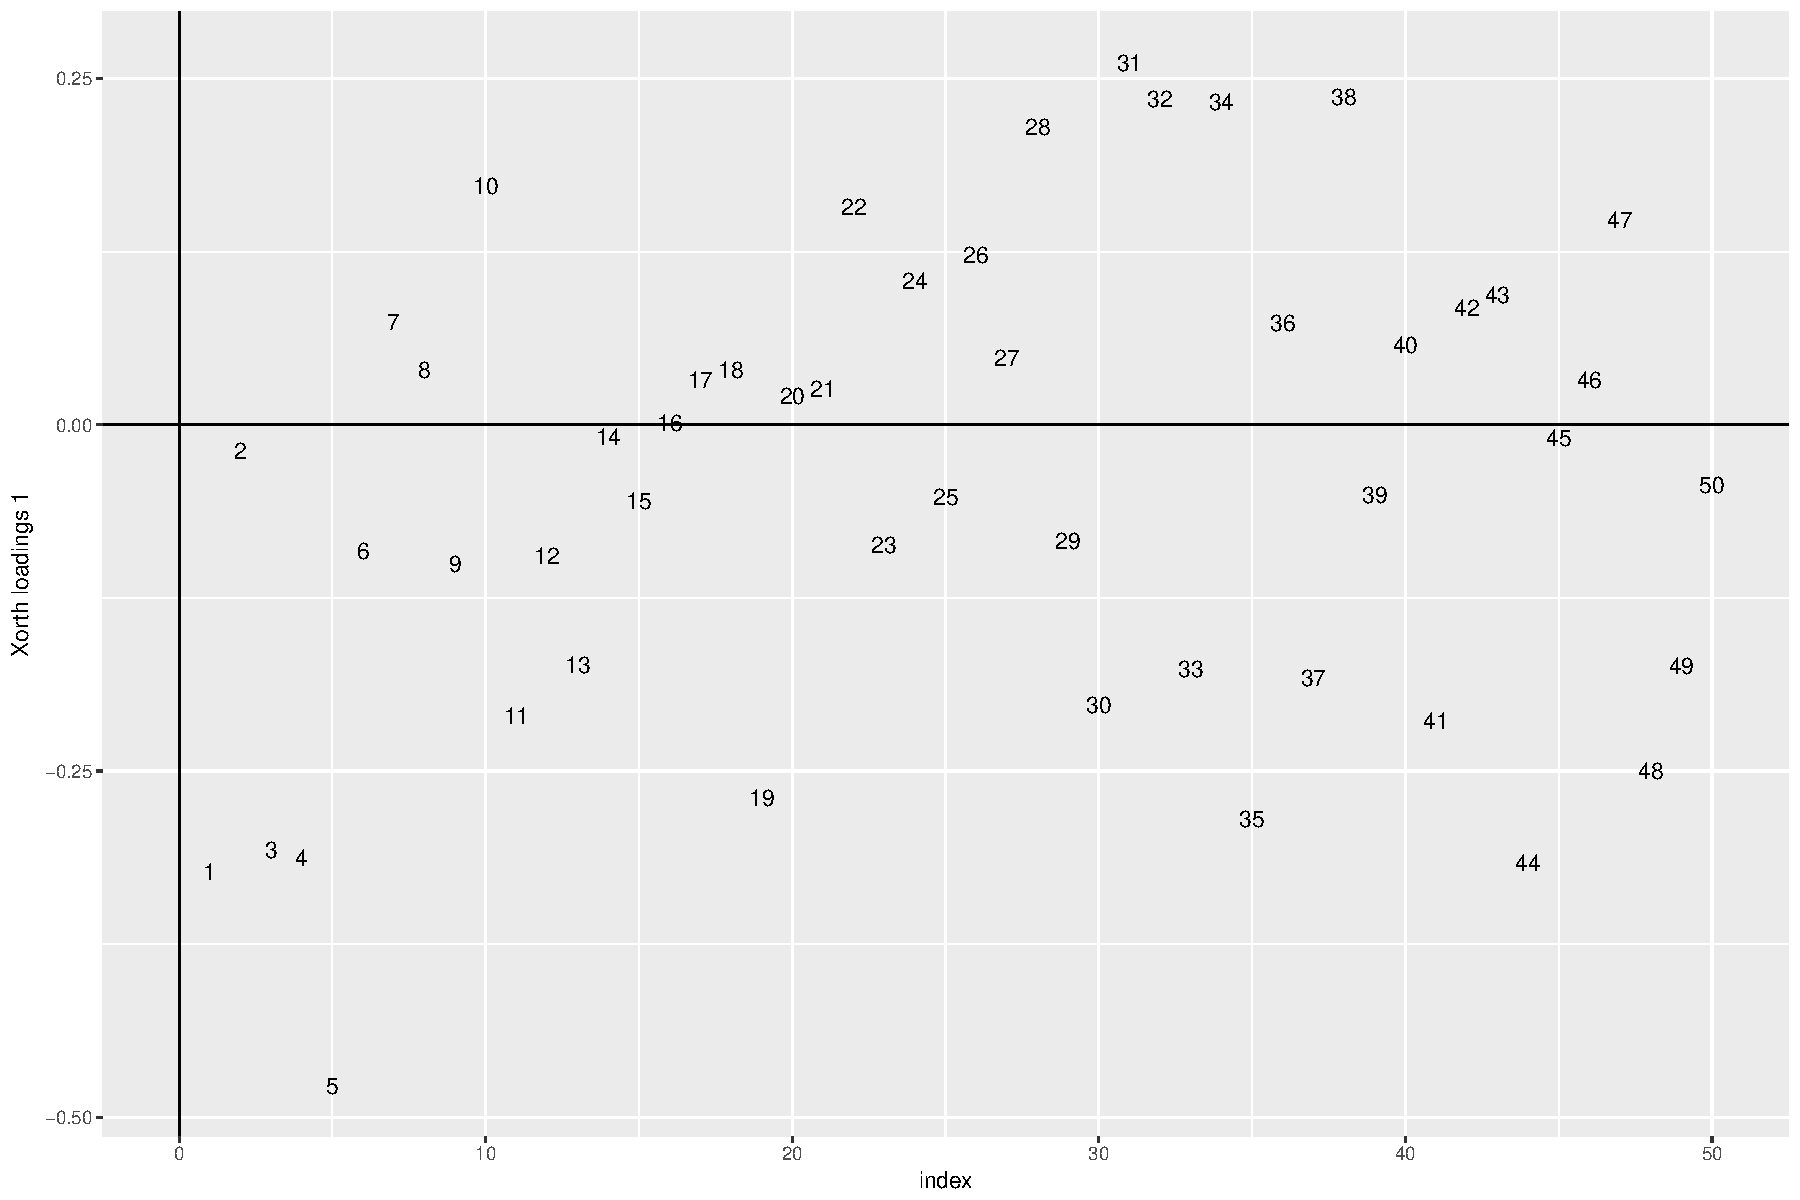
\includegraphics{Figs/unnamed-chunk-6-1.pdf}


\end{document}
